\documentclass{beamer}\usepackage[]{graphicx}\usepackage[]{color}
% maxwidth is the original width if it is less than linewidth
% otherwise use linewidth (to make sure the graphics do not exceed the margin)
\makeatletter
\def\maxwidth{ %
  \ifdim\Gin@nat@width>\linewidth
    \linewidth
  \else
    \Gin@nat@width
  \fi
}
\makeatother

\definecolor{fgcolor}{rgb}{0.345, 0.345, 0.345}
\newcommand{\hlnum}[1]{\textcolor[rgb]{0.686,0.059,0.569}{#1}}%
\newcommand{\hlstr}[1]{\textcolor[rgb]{0.192,0.494,0.8}{#1}}%
\newcommand{\hlcom}[1]{\textcolor[rgb]{0.678,0.584,0.686}{\textit{#1}}}%
\newcommand{\hlopt}[1]{\textcolor[rgb]{0,0,0}{#1}}%
\newcommand{\hlstd}[1]{\textcolor[rgb]{0.345,0.345,0.345}{#1}}%
\newcommand{\hlkwa}[1]{\textcolor[rgb]{0.161,0.373,0.58}{\textbf{#1}}}%
\newcommand{\hlkwb}[1]{\textcolor[rgb]{0.69,0.353,0.396}{#1}}%
\newcommand{\hlkwc}[1]{\textcolor[rgb]{0.333,0.667,0.333}{#1}}%
\newcommand{\hlkwd}[1]{\textcolor[rgb]{0.737,0.353,0.396}{\textbf{#1}}}%
\let\hlipl\hlkwb

\usepackage{framed}
\makeatletter
\newenvironment{kframe}{%
 \def\at@end@of@kframe{}%
 \ifinner\ifhmode%
  \def\at@end@of@kframe{\end{minipage}}%
  \begin{minipage}{\columnwidth}%
 \fi\fi%
 \def\FrameCommand##1{\hskip\@totalleftmargin \hskip-\fboxsep
 \colorbox{shadecolor}{##1}\hskip-\fboxsep
     % There is no \\@totalrightmargin, so:
     \hskip-\linewidth \hskip-\@totalleftmargin \hskip\columnwidth}%
 \MakeFramed {\advance\hsize-\width
   \@totalleftmargin\z@ \linewidth\hsize
   \@setminipage}}%
 {\par\unskip\endMakeFramed%
 \at@end@of@kframe}
\makeatother

\definecolor{shadecolor}{rgb}{.97, .97, .97}
\definecolor{messagecolor}{rgb}{0, 0, 0}
\definecolor{warningcolor}{rgb}{1, 0, 1}
\definecolor{errorcolor}{rgb}{1, 0, 0}
\newenvironment{knitrout}{}{} % an empty environment to be redefined in TeX

\usepackage{alltt}[handout]

\usepackage{verbatim, amsmath,amssymb}
\usepackage[font = small]{caption}
\usepackage{pgf}
\usepackage{tikz}
\usetikzlibrary{arrows,automata}
\usetikzlibrary{positioning}
%\usepackage{natbib}
%\usepackage[backend=bibtex]{biblatex}
%\usepackage{natbib}
%\usepackage{mathrsfs,fancyhdr,syntonly,lastpage,hyperref,enumitem,graphicx,wrapfig, subcaption}

\usefonttheme[onlymath]{serif}

\usetheme{AnnArbor}
\usecolortheme{beaver}

\setlength{\unitlength}{\textwidth}  % measure in textwidths
\usepackage[normalem]{ulem}

\setbeamertemplate{navigation symbols}{}
\setbeamertemplate{enumerate items}[default]
\setbeamertemplate{enumerate subitem}{\alph{enumii}.}
\setbeamertemplate{enumerate subsubitem}{\roman{enumiii}.}
\setkeys{Gin}{width=0.6\textwidth}

\AtBeginSection[]{
  \begin{frame}
  \vfill
  \centering
  \begin{beamercolorbox}[sep=8pt,center,shadow=true,rounded=true]{title}
    \usebeamerfont{title}\insertsectionhead\par%
  \end{beamercolorbox}
  \vfill
  \end{frame}
}

\AtBeginSubsection{}

\title{Inducing Point GP Approximations}
%\institute[Iowa State]{Iowa State University}
\date{\today}

%\newcommand{\mG}{\mathrm{\Gamma}}
%\newcommand{\I}{\mathrm{I}}
%\newcommand{\mySigma}{\mathrm{\Sigma}}
%\newcommand{\ind}{\stackrel{ind}{\sim}}
\DeclareMathOperator*{\argmax}{argmax}
\DeclareMathOperator*{\argmin}{argmin}

\graphicspath{{figures/}} % path containing figures must be in the folder where the tex file is located
\setbeamertemplate{caption}[numbered]
\IfFileExists{upquote.sty}{\usepackage{upquote}}{}
\begin{document}
%\SweaveOpts{concordance=TRUE}


\frame{\maketitle}

\frame{\frametitle{Motivating Example}
\centering
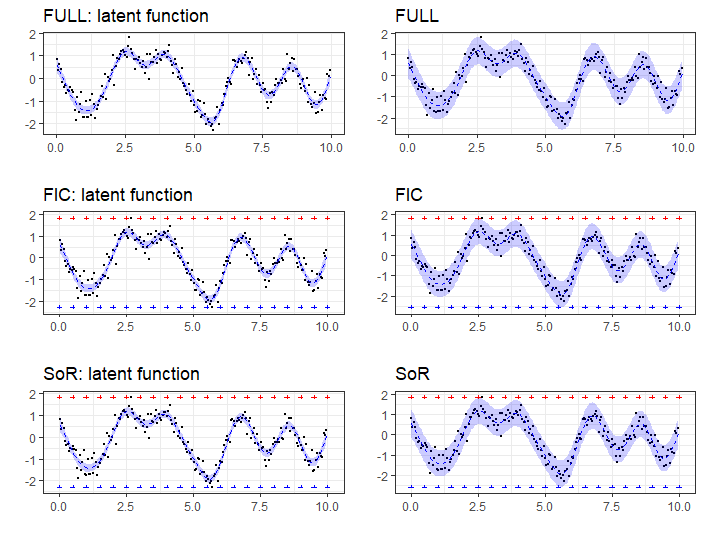
\includegraphics{figures/sparse_vs_full_example_good}
}

\frame{\frametitle{GP Notation}
\[ \phi \sim \mathcal{GP}(m(\cdot), k_{\theta}(\cdot, \cdot)) \] 
\begin{itemize}
  \item $y$: vector of observed response values
  \item $x_i$: vector of explanatory variables for response value $y_i$ 
  ($x$ is the matrix with $x_i$ as rows)
  \item $\tilde{x}$: matrix of inducing point locations with rows $\tilde{x}_i$
  %\item $m(\cdot)$: mean function 
  %\item $k_{\theta}(\cdot, \cdot)$: covariance function 
  \item $f_i = f(x_i)$: realized values of the latent function at $N$ input locations $x_i \in \mathcal{X} \subset \mathbb{R}^d$ 
  \item $f_x$: vector of (realized) $N$ function values at observed data locations 
  \item $\phi_x \sim \mathcal{N}\left(m_x, \Sigma_{xx} \right)$ 
\end{itemize}
}

\frame{\frametitle{Subset of Regressors (SoR) Approximation}
\begin{itemize} 
\item $p_{SoR}(\phi_x,\phi_{\tilde{x}})  = p(\phi_x,\phi_{\tilde{x}})  = p(\phi_x|\phi_{\tilde{x}})p(\phi_{\tilde{x}})$ 
  \begin{itemize}
    \item $\phi_x|\phi_{\tilde{x}} \sim N\left( m_x + \Sigma_{x\tilde{x}} \Sigma_{\tilde{x}\tilde{x}}^{-1}(\phi_{\tilde{x}} - m_{\tilde{x}}) , 0 \right)$ 
    \item $\phi_{\tilde{x}} \sim \mathcal{N}(m_{\tilde{x}}, \Sigma_{\tilde{x}\tilde{x}})$ 
  \end{itemize}
\end{itemize}
}

\frame{\frametitle{Fully Independent Conditional (FIC) Approximation}
\begin{itemize} 
  \item $p_{FIC}(\phi_x,\phi_{\tilde{x}})  = p(\phi_x,\phi_{\tilde{x}})  = p(\phi_x|\phi_{\tilde{x}})p(\phi_{\tilde{x}})$ 
  \begin{itemize}
    \item $\phi_x|\phi_{\tilde{x}} \sim N\left( m_x + \Sigma_{x\tilde{x}} \Sigma_{\tilde{x}\tilde{x}}^{-1}(\phi_{\tilde{x}} - m_{\tilde{x}}) , \text{diag}\left[ \Sigma_{xx} - \Sigma_{x\tilde{x}} \Sigma_{\tilde{x}\tilde{x}}^{-1} \Sigma_{\tilde{x}x}  \right] \right)$ 
    \item $\phi_{\tilde{x}} \sim \mathcal{N}(m_{\tilde{x}}, \Sigma_{\tilde{x}\tilde{x}})$ 
  \end{itemize}
\end{itemize}
}

\frame{\frametitle{Changing the approximation for predictions}
\begin{itemize} 
  \item $x^*_i$: vector of explanatory variables for test set observation $i$
  \item Projected Process Approximation (PPA) / Deterministic Training Conditional (DTC)
  \item Fully Independent Training Conditional (FITC)
  \item $\phi_{x}^*|\phi_{\tilde{x}} \sim  \mathcal{N}\left( m_{x^*} + \Sigma_{x^*\tilde{x}} \Sigma_{\tilde{x}\tilde{x}}^{-1}(\phi_{\tilde{x}} - m_{\tilde{x}}) , \Sigma_{x^*x^*} -  \Sigma_{x^*\tilde{x}} \Sigma_{\tilde{x}\tilde{x}}^{-1}\Sigma_{\tilde{x} x^*} \right)$
\end{itemize}
}

\frame{\frametitle{Summary of Inducing Point Methods}

Do the following quantities match the full GP?
\begin{table}
\begin{tabular}{|c|c|c|c|}
\hline
%& $V_{sparse}\left[ \phi_{x_i} \right] = V_{full}\left[ \phi_{x_i} \right]$ &
%$V_{sparse}\left[ \phi_{x^*} \right] = V_{full}\left[ \phi_{x^*} \right]$ \\
& Training variances & Test variances & Test covariances \\ 
\hline
SoR & NO & YES & NO \\
PPA/DTC & NO & YES & YES\\
FIC & YES & YES & NO \\
FITC & YES & YES & YES \\
\hline
\end{tabular}
\end{table}

In a single layer GP, the \emph{posterior approximation} used in 
Damianou and Lawrence is the \emph{same} as that resulting from the PPA/DTC model.
}

\frame{\frametitle{Summary of Inducing Point Methods (cont.)}
\begin{itemize}
\item All methods result in conditional independence of $\phi_{x_i}|\phi_{\tilde{x}}$, so 
no sparse method defines the same prior covariances on the \emph{training set} as
the full GP.
\item Posterior predictive variances/covariances are different for all methods.
\item Changing the prior for \emph{only} the variances / covariances on the test set
does \emph{not} change the posterior predictive mean.
\end{itemize}
}


\frame{\frametitle{Model Comparison when K is too small}
\centering
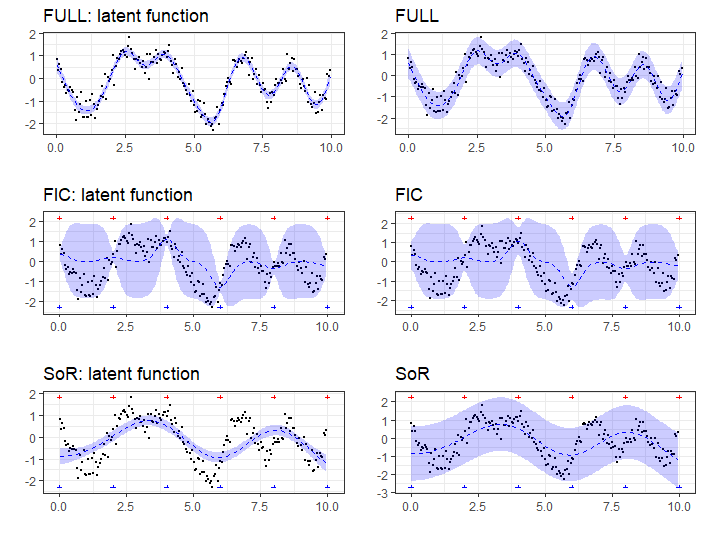
\includegraphics{figures/sparse_vs_full_example_bad}
}

\frame{\frametitle{Fitting models with likelihood optimization}
PPA/DTC and SoR both use the \emph{same} likelihood, so fitted paramters 
will be the same. The same goes for FIC and FITC. So what?

\begin{itemize}
 \item SoR and PPA/DTC overestimate noise variance to compensate for
 lack of model flexibility/poorly approximated marginal function variances. 
 \emph{If} the PPA/DTC ``correction" fixes the posterior function 
 variance, the PPA/DTC models \emph{must} overestimate posterior variance of the response variables. 
 \item FIC and FITC do not share this relationship, but there may be undesirable
 consequences in terms of the posterior covariances.
\end{itemize}

}

\begin{frame}

\begin{thebibliography}{10}
\bibitem{candela2005}
\alert{Joaquin Qui\~nonero-Candela and Carl Edward Rasmussen}
\newblock{A Unifying View of Sparse Approximate Gaussian Process Regression}
\newblock{\em Journal of Machine Learning Research, 2005, 6, 1939-1959}.

\bibitem{titsias2009}
\alert{Michalis K. Titsias}
\newblock{Variational Learning of Inducing Variables in Sparse Gaussian Processes}
\newblock{In {\em Artificial Intelligence and Statistics, 2009, 567-574} }.

\bibitem{titsias2009b}
\alert{Michalis K. Titsias}
\newblock{Variational Model Selection for Sparse Gaussian Process Regression}
\newblock{Technical report, School of Computer Science, University of Manchester, 2009}.
\end{thebibliography}

\end{frame}

\end{document}
